\documentclass{article}
\usepackage{listings}
\usepackage{amsmath}
\usepackage{fullpage}
\usepackage{tabularx}
\usepackage{graphicx}
\usepackage{tikz}
\usetikzlibrary{shapes.geometric, arrows}
\usepackage{cite}
\usepackage{hyperref}
\begin{document}
\lstset{language=python, tabsize=4}
\title{Node embedding}
\author{Yuchen Hou}
\maketitle

\begin{abstract}
	I summarize recent deep learning approaches in graph mining and identify the key process in all these approaches: node embedding(the process of representing every node in the graph with a 1D numerical array called node vector, i.e. embedding nodes in node space). Every node vector contains information about the node related to the prediction task. This process is critical because neural nets can only handle numerical variables directly, which means everything nonnumerical needs to be converted to numbers before it can be processed by a neural net. Other aspects in these approaches are task specific and I will address them in corresponding sections.
\end{abstract}

\section{Introduction}

\subsection{Deep learning in different domains}
Deep learning architectures built from neural nets have achieved wide spread success in 3 domains: speech recognition\cite{hannun2014deep}, image recognition\cite{simonyan2014very}, and natural language processing\cite{yao2013recurrent}. In order to understand how it can handle prediction tasks in graph mining, first we take an overview on 3 types entities in these 3 domains and in graph mining. \autoref{tab:domains} provides a summary of these entities, their representations in neural nets and inter-entity relation examples in these domains.
\begin{table}[h]
	\centering
	\begin{tabularx}{\textwidth}{ |c|c|c|X| }
		\hline domain & entity & representation & relations to other entities \\ 
		\hline image recognition & image & 2D pixel array & NA \\ 
		\hline speech recognition & utterance & 2D spectrogram array & NA \\ 
		\hline natural language processing & word & word vector(1D array) & relations to other words \\ 
		\hline graph mining & movie & node vector(1D array) & directed by director, etc \\ 
		\hline graph mining & user & node vector(1D array) & rate movies, message other users, etc \\ 
		\hline graph mining & article & node vector(1D array) & address topics, cite other articles, etc \\
		\hline
	\end{tabularx}
	\caption{A summary of various types of entities, their representations and inter-entity relations in different domains: images and utterances can be directly represented by 2D numerical arrays, but have no strong relations to other images or utterances; words and various types of nodes in graphs are  represented by 1D numerical arrays(which will be introduced below), and have strong relations to other words and nodes. Notice that the representations for all the entities are numerical arrays, because neural nets rely on neurons' activations and communications, which are both numerical.}
	\label{tab:domains}
\end{table}

\subsection{Entity representations in different domains}
In \autoref{tab:domains}, the entities listed in the lower rows have increasing representation complexities. Pixel and spectrogram arrays for images and utterances can be measured by physical instruments from the entities themselves. \autoref{fig:Airy-pattern} shows how an image is represented by a 2D pixel intensity array in image recognition. \autoref{fig:Spectrogram-19thC} shows how an utterance is represented by a 2D spectrogram array in speech recognition. Notice that beside the differences in their axes, these 2 representations have little difference. This direct way to represent images and utterances with numerical arrays makes it easy for neural net to process them. If words and nodes can be represented by numerical arrays in a similar way, neural nets will be able to handle challenging prediction tasks in these 2 domains as well. Now the question is how to achieve this representation. Interestingly, it turns out neural net itself has the capability to do it.
\begin{figure}[h]
	\centering
	\includegraphics[width=0.5\linewidth]{Airy-pattern}
	\caption{The 2D pixel array of an image of  \href{https://commons.wikimedia.org/wiki/File:Airy-pattern.svg}{the airy pattern} (John Doe / Wikimedia Commons / Public Domain): the horizontal and vertical axes represent the width and the height; the numerical value at a specific (width, height) location is normalized pixel intensity in range(0, 1).}
	\label{fig:Airy-pattern}
\end{figure}
\begin{figure}[h]
	\centering
	\includegraphics[width=\linewidth]{Spectrogram-19thC}
	\caption{The 2D spectrogram array of \href{https://commons.wikimedia.org/wiki/File:Spectrogram-19thC.png}{a male voice saying [nineteenth century]}(Aquegg / Wikimedia Commons / Public Domain): the horizontal and vertical axes represent the time and frequency; the numerical value at a specific (time, frequency) location is the sound intensity measured in unit dBFS(decibel relative to full scale).}
	\label{fig:Spectrogram-19thC}
\end{figure}

\subsection{Objectives}
In the next few sections I summarize recent neural net approaches in natural language processing and graph mining, especially their key processes: word embedding and node embedding. I mainly focus on a specific approach call DeepWalk introduced in \cite{perozzi2014deepwalk} (the term "the paper" refers to this paper in the following context). I also introduce a new node embedding process with strengths in low complexity, comprehensive learning, and multi-task prediction.

\section{Word embedding}
In this section, I summarize word embedding(representing every word in a vocabulary with a word vector) introduced in \cite{mikolov2013efficient}, which is used as the foundation of node embedding in the paper.

\subsection{The goal}
We want to represent each word in the vocabulary with a word vector, so that a neural net can use it to perform prediction tasks in natural language processing like language modeling. Word vectors are more difficult to get compared to 2D arrays of images and utterances. This is because no instrument can measure words and produce the vector - they can only be learned from its relations to other words in the corpus. \autoref{tab:word} shows how each word in a vocabulary is represented by a word vector.
\begin{table}[h]
	\centering
	\begin{tabularx}{0.5\textwidth}{|c|c|X|} \hline
		rank & word & word vector \\ \hline
		1 & the & [2.3, 564, -9.5 ... 3] \\ \hline
		2 & be & [76, -342.2, 0.3 ... 4.2] \\ \hline
		3 & to & [-345, -834, 0.3 ... 34] \\ \hline
		... & ... & ... \\ \hline
		n & $ word_n $ & $ [x_1, x_2, x_3 ... x_d] $ \\ \hline
	\end{tabularx}
	\caption{Word vectors sorted by the popularity of the words in English: there are n words in the entire vocabulary; each word is represented by a vector of size d; each vector's numerical values in this table are hypothetical, which will be learned in real applications.}
	\label{tab:word}
\end{table}

\subsection{Application scenario}
Once word embedding is accomplished, neural nets can use the resulting word vectors to perform prediction tasks. The application discussed in the paper is language modeling. The dataset is a corpus in which every word can be any one of the n words in a finite vocabulary. The prediction task is: given a sequence X of t words, predict the next word Y. In other words, both X and Y can be viewed as random variables and we want to find the conditional probability:
\begin{equation}
P(Y = w_t|X = (w_0, w_1, w_2 ... w_{t-1}))
\end{equation}
where w's are words indexed by their ordering in the sequence. In the simpler case, we don't want to find the above possibility for every word; we only want to find the word that has the maximum possibility:
\begin{equation}
	w = argmax_{w_t}P(Y = w_t|X = (w_0, w_1, w_2 ... w_{t-1}))
\end{equation}

\subsection{Observations and the approach}
It's easy to see why word vectors can be learned from relations between words manifested in their co-occurrences within a corpus. In any word sequence, the term context refers the surrounding words of word w within certain distances. For example, the sequence [guard, peace, and, justice, in, the, universe] has the following word and context of radius 3:
\begin{itemize}
	\item sequence = [guard, peace, and, justice, in, the, universe]
	\item word = [justice]
	\item context of radius 3 = [guard, peace, and, in, the, universe]
\end{itemize}
Every word in the context is related to [justice] in some way and these relations provide information about it. For example, [guard] describes its attribute of existing condition: justice exists if there are those who protect it; otherwise evil will destroy it. As another example, [peace] describes its attribute of virtue: justice is morally good and desirable, like peace. Now it's very clear that words in the context of a word w provides information about different attributes of w. A stronger statement is: every word w can be defined by words in all its contexts within the corpus. In fact, this is also how exactly every dictionary defines words - describing a word using other related words. The previous example sequence is actually part of a complete definition of the word [Jedi] provided by Google Dictionary: [a member of the mystical knightly order in the Star Wars films, trained to guard peace and justice in the universe]. Apparently, we can understand this phenomenon in 2 ways:
\begin{enumerate}
	\item words in the contexts of a word describe its relations with other words
	\item words in the contexts of a word describe its attributes
\end{enumerate}
No matter which one is better, we have the observation that related words provide all the information about a word we can possibly get from a corpus. Therefore, it's a good idea to learn the word vector for each word supervised by the words in its contexts.

\subsection{Implementation}

\subsubsection{Skip-gram model}
The paper uses skip-gram neural net model to learn the word vectors. In order to take advantage of large corpora, skip-gram model trades off some accuracy for high learning speed by minimizing its neural net complexity to only 3 fully connected layers with formation [n, d, n], where n is the vocabulary size and d is the embedding size. An example model with n=8 and d=4 is shown in \autoref{fig:skipGram}. In fact, skip-gram model is a shallow neural net. The ith unit in the embedding layer has linear activation function:
\begin{equation}
	y_i = f_i(x) = v_i \cdot x
	\label{eq:linear}
\end{equation}
where $ v_i $ and x are the weight vector and the input vector with size n. The ith unit in the output layer has softmax activation function (generalized from multi-class logistic regression):
\begin{equation}
	y_i = f_i(x) = \frac{exp(v_i \cdot x)}{\sum_{i = 1}^{n}exp(v_i \cdot x)}
\end{equation}
where $ v_i $ and x are the weight vector and the input vector with size d. Notice that these symbols are not related to those in \autoref{eq:linear}. Also notice that although $ f_i(x) $ is not easily implementable. What I show here is a conceptual illustration - the real implementation has more optimized and complex structure.

\begin{figure}[h]
	\centering
	\newcommand{\layersep}{2.5cm}
	\newcommand{\vocabularySize}{8}
	\newcommand{\embeddingSize}{4}
	\begin{tikzpicture}[shorten >=1pt,->,draw=black!50, node distance=\layersep]
	\tikzstyle{every pin edge}=[<-,shorten <=1pt]
	\tikzstyle{neuron}=[circle,fill=black!25,minimum size=17pt,inner sep=0pt]
	\tikzstyle{input neuron}=[neuron, fill=green!50];
	\tikzstyle{output neuron}=[neuron, fill=red!50];
	\tikzstyle{hidden neuron}=[neuron, fill=blue!50];
	\tikzstyle{annot} = [text width=4em, text centered]
	
	% Draw the input layer
	\foreach \name / \y in {1,...,\vocabularySize}
	% This is the same as writing \foreach \name / \y in {1/1,2/2,3/3,4/4}
	\node[input neuron, pin=left:$ w_\y $] (I-\name) at (0,-\y) {};
	
	% Draw the hidden layer
	\foreach \name / \y in {1,...,\embeddingSize}
	\path[yshift=-2cm]
	node[hidden neuron] (H-\name) at (\layersep,-\y cm) {};
	
	% Draw the output layer
	\foreach \name / \y in {1,...,\vocabularySize}
	\node[output neuron, pin={[pin edge={->}]right:$ w_\y $}] (O-\name) at (2*\layersep,-\y) {};
	
	% Connect the input layer with the hidden layer
	\foreach \source in {1,...,\vocabularySize}
	\foreach \dest in {1,...,\embeddingSize}
	\path (I-\source) edge (H-\dest);
	
	% Connect the hidden layer with the output layer
	\foreach \source in {1,...,\embeddingSize}
	\foreach \dest in {1,...,\vocabularySize}
	\path (H-\source) edge (O-\dest);
	
	% Annotate the layers
	\node[annot,above of=H-2] {embedding layer};
	\node[annot,above of=I-2] {input layer};
	\node[annot,above of=O-2] {output layer};
	\end{tikzpicture}
	
	\caption{The skip-gram model with vocabulary size 8 and embedding size 4: the model consists of only 3 layers - an input layer with one-hot activation, an embedding layer of linear units, and an output layer of softmax units. For example, given sequence = [$ w_3, w_2, w_8, w_1, w_4 $], we have input word = [$ w_8 $] and output context = [$ w_1, w_2, w_3, w_4 $]. The input layer has activation x = (0, 0, 0...0, 1), where $ w_8 $ is 1 and others are 0; the output layer has activation y = (1, 1, 1, 1, 0 ... 0), where $ w_1, w_2, w_3, w_4 $ are 1 and others are 0. The weights in the embedding layer are the word vectors shown in \autoref{tab:word}. For example, the word vector for $ w_8 $ are the weights in the embedding layer units connected to $ w_8 $ These weights are randomly initialized and learned by the neural net during training. The embedding layer's activation is equal to the word vector of the current word due to one-hot activation in the input layer.}
	\label{fig:skipGram}
\end{figure}

\subsubsection{Loss function}
The paper uses the common loss function for classification models with softmax output layer - the cross entropy loss:
\begin{equation}
loss = H(t, y) = - \sum_{i = 1}^{n} t_i log(y_i)
\end{equation}
where t is the expected output provided by the training data and y is the actual output predicted by the model.

\subsubsection{Learning algorithm}
The paper uses the standard learning algorithm for neural net: stochastic gradient descent with back propagation\cite{lecun2012efficient}.

\subsection{Learning outcome}
The word embedding process can produce word vectors that capture semantic information about words. There are 2 useful and interesting properties about these word vectors:
\begin{enumerate}
	\item the distance between 2 word vectors represents the semantic similarity between the 2 words, e.g., $ \mid vector(university) - vector(college) \mid < \mid vector(university) - vector(kingdom) \mid $;
	\item the difference of 2 word vectors represents the semantic relation of the 2 words, e.g., $ \mid vector(king) - vector(man) \mid < \mid vector(queen) - vector(woman) \mid $;
\end{enumerate}
There are nice visualizations demonstrated by Tensor Flow project in their \href{https://www.tensorflow.org/versions/r0.7/tutorials/word2vec/index.html}{word2vec tutorial}.

\section{Node embedding}
In this section, I summarize node embedding(representing every node in a graph with a node vector) introduced in \cite{perozzi2014deepwalk}.

\subsection{The goal}
The goal of node embedding is identical to word embedding: to represent nodes with node vectors so that a neural net can use it. Similar to word vectors shown in \autoref{tab:word}, node vectors are shown in \autoref{tab:node}.
\begin{table}[h]
	\centering
	\begin{tabularx}{0.5\textwidth}{|c|c|X|} \hline
		ID & node & node vector \\ \hline
		1 & A & [2.3, 564, -9.5 ... 3] \\ \hline
		2 & B & [76, -342.2, 0.3 ... 4.2] \\ \hline
		3 & C & [-345, -834, 0.3 ... 34] \\ \hline
		... & ... & ... \\ \hline
		n & $ node_n $ & $ [x_1, x_2, x_3 ... x_d] $ \\ \hline
	\end{tabularx}
	\caption{Node vectors sorted by the node ID in a graph: there are n nodes in the entire graph; each node is represented by a vector of size d; each vector's numerical values in this table are hypothetical, which will be learned in real applications.}
	\label{tab:node}
\end{table}

\subsection{Application scenario}
Once node embedding is accomplished, neural nets can use the resulting node vectors to perform prediction tasks. The application mentioned in the paper is node classification. The dataset is a graph in which links do not have attributes but every node can have any number of the n labels in a finite label set. More formally, every node has one attribute - a list of n boolean variables where each variable indicates whether the node has a particular label. For example,
\begin{lstlisting}
node[4].attribute = [ture, false, false... true]
\end{lstlisting}
means $ node_4 $ has $ label_0 $, has no $ label_1 $, has no $ label_2 $... and has $ label_n $. The attribute values are known for a portion of nodes, which serve as training data. The prediction task is: given a node X, predict its attribute value Y(determine which labels it has).

\subsection{Observations and the approach}
By comparing the data in natural language processing and that in graph mining, we can observe their similarities, shown in \autoref{tab:wordVSnode}. Most importantly, a sentence is very similar to a walk.
\begin{table}[h]
	\centering
	\begin{tabularx}{\textwidth}{ |X|X|X| } \hline
		aspect  & natural language processing & graph mining \\ \hline
		information source & text & graph \\ \hline
		basic entities & words & nodes \\ \hline
		entity collection & vocabulary & node set \\ \hline
		relational data source & collocations (implicit) & links (explicit) \\ \hline
		entity sequences & sentences & random walks \\ \hline
	\end{tabularx}
	\caption{A comparison of natural language processing and graph mining from several aspects: the similarity of these 2 domains across all these aspects makes it possible to develop node embedding process based on word embedding.}
	\label{tab:wordVSnode}
\end{table}
As neural nets can represent every word in a vocabulary based on the relations between words in word sequences in natural languages (sentences), in the same way it should be able to represent every node in the node set based on the links between nodes in node sequences in the graph (random walks). Based on these observations, the node vectors can be learned supervised by the nodes in the random walk.

\subsection{Implementation}
The paper implement node embedding the same way as word embedding discussed in previous section, which won't be repeated here. The node sequences are random walks sampled from the graph. After the model finishes the node embedding learning stage, it replaces the softmax units in the output layer with logistic regression units to learn to perform label prediction task. During this learning stage, only the output layer updates its weights during the learning, while the embedding layer maintains its weights learned during the previous stage. Otherwise, the learned node vectors will be destroyed. Its neural net has 3 fully connected layers with formation [n, d, l], where n is the node set size, d is the embedding size and l is the label set size. An example model with n=8, d=4 and l=2 is shown in \autoref{fig:label}. This model is a shallow neural net. The ith unit in the output layer has logistic regression activation function:
\begin{equation}
y_i = f(x) = \frac{1}{1 + exp(-v_i \cdot x)}
\end{equation}
where $ v_i $ and x are the weight vector and the input vector with size d.
\begin{figure}[h]
	\centering
	\newcommand{\layersep}{2.5cm}
	\newcommand{\vocabularySize}{8}
	\newcommand{\embeddingSize}{4}
	\newcommand{\labelSetSize}{2}
	\begin{tikzpicture}[shorten >=1pt,->,draw=black!50, node distance=\layersep]
	\tikzstyle{every pin edge}=[<-,shorten <=1pt]
	\tikzstyle{neuron}=[circle,fill=black!25,minimum size=17pt,inner sep=0pt]
	\tikzstyle{input neuron}=[neuron, fill=green!50];
	\tikzstyle{output neuron}=[neuron, fill=red!50];
	\tikzstyle{hidden neuron}=[neuron, fill=blue!50];
	\tikzstyle{annot} = [text width=4em, text centered]
	
	% Draw the input layer
	\foreach \name / \y in {1,...,\vocabularySize}
	% This is the same as writing \foreach \name / \y in {1/1,2/2,3/3,4/4}
	\node[input neuron, pin=left:$ node_\y $] (I-\name) at (0,-\y) {};
	
	% Draw the hidden layer
	\foreach \name / \y in {1,...,\embeddingSize}
	\path[yshift=-2cm]
	node[hidden neuron] (H-\name) at (\layersep,-\y) {};
	
	% Draw the output layer
	\foreach \name / \y in {1,...,\labelSetSize}
	\node[output neuron, pin={[pin edge={->}]right:$ label_\y $}] (O-\name) at (2*\layersep,-\y-3) {};
	
	% Connect the input layer with the hidden layer
	\foreach \source in {1,...,\vocabularySize}
	\foreach \dest in {1,...,\embeddingSize}
	\path (I-\source) edge (H-\dest);
	
	% Connect the hidden layer with the output layer
	\foreach \source in {1,...,\embeddingSize}
	\foreach \dest in {1,...,\labelSetSize}
	\path (H-\source) edge (O-\dest);
	
	% Annotate the layers
	\node[annot,above of=H-2] {embedding layer};
	\node[annot,above of=I-2] {input layer};
	\node[annot,above of=O-2] {output layer};
	\end{tikzpicture}
	\caption{The label prediction model with node set size 8, embedding size 4 and label set size 2: the model consists of only 3 layers - an input layer with one-hot activation, an embedding layer of linear units, and an output layer of logistic regression units. For example, given input node = [$ node_8 $] and output label = [$ label_1 $]. The input layer has activation = (0, 0, 0...0, 1), where $ w_8 $ is 1 and others are 0; the output layer has activation = (1, 0), where $ label_1 $ is 1 and $ label_2 $ is 0. The weights in the embedding layer are the node vectors shown in \autoref{tab:node}. In this stage, the units in embedding layer already have all node vectors learned and will not update the weights; only the unites in output layer will update their weights.}
	\label{fig:label}
\end{figure}

\subsection{Strengths of this approach}

\subsubsection{Representing nodes as node vectors}
This fits many real world graphs well: usually a graph has complex entities with unobservable attributes which we represent as nodes; it also has simple interactions/relations between these entities with observable attributes which we represent as links, as shown in \autoref{tab:nodesVSlinks}. In terms of information flow, we can understand this approach of graph mining as a node-centric approach, as information about nodes is extracted from links connecting these nodes and then stored in nodes. In a social network scenario where we want to understand a user, this means who a user contacts and what a user does tells us what kind of person he is.
\begin{table}[h]
	\centering
	\begin{tabularx}{0.5\textwidth}{ |c|c|X| } \hline
		aspect  & node & link \\ \hline
		complexity & high & low \\ \hline
		attribute observability & low & high \\ \hline
	\end{tabularx}
	\caption{A comparison of node and link with respect to their complexity and attribute observability: links tend to have low complexity and high attribute observability while nodes are the opposite. In a social network example, it's easy to observe simple user activities like sending messages other users, leaving comments on posts and give ratings to music, but it's hard to observe complex user attributes like personality, style or taste in music.}
	\label{tab:nodesVSlinks}
\end{table}

\subsubsection{Online learning}
This fits streaming graph scenarios, when it is sufficient to keep a finite number of latest links streamed in inside the memory, just enough to sample walks of reasonable lengths. The training samples in this approach are walks in the graph. Every walk is randomly generated, then fed to the neural net. During this training step, the neural net extracts the information provided by this walk and uses it to update the node vector. After this training step,  the random walk can be discarded. Therefore, the learning is incremental and only requires samples of different walks in the graph, not the construction or storage of the complete graph.

\subsection{Weaknesses of this approach}

\subsubsection{Node sequence generation}
The node sequence generation with random walks on the graph is likely a weakness, although these sequences shares 3 similarities with word sequences used by very successful skip-gram model. These similarities are listed below with explanations of the weakness:
\begin{enumerate}
	\item Sentences and walks are both very natural sequences. Skip-gram model uses sentences because they are the only available data in corpora, not because this provides special benefits to the model. Furthermore, most of the words in the context of a word are usually related to it so using sentences doesn't have much negative effect to skip-gram. However, the situation is not the same for walks in graph. First, sampling nodes from long walks in the graph is not the only option; a more computational efficient one is to sample nodes from the neighborhood of the node. Also, a deep walk is likely to sample remote nodes, which are not strongly related to the root node.
	\item Words and nodes in the sequences have informative ordering. Although the ordering is significant in both cases, they are 2 different types of orderings. In a sentence, words are ordered to make the sentence correct and meaningful, not to make more similar words closer to each other. For example, in sentence [The quick brown fox jumps over the lazy dog.], [quick] and [brown] are very close but they are in fact very unrelated words; [fox] and [dog] are very far but they are strongly related words. Fortunately, this undesirable phenomena doesn't have negative effect on skip-gram model, because skip-gram model ignores word ordering anyway. This is not the case in a node sequence, where nodes with closer distances in the graph usually have closer distances in the sequence. This ordering is very critical and contains information we want skip-gram model to capture, but its indifference to ordering makes this impossible.
	\item The frequency distributions of words and nodes follow power law. This one is bad for both cases, which should be avoided instead of taken advantage of. For example, skip-gram model can get useful information from co-occurrences of 'capital' and 'Beijing', but not so much from co-occurrences of 'the' and 'capital'. Here 'the' is a prominent example word with very high frequency but provides little information about anything. Frequent words like 'the' reduce both the speed and accuracy of learning word embedding, and are intentionally discard with sub-sampling technique in natural language processing \cite{mikolov2013distributed}.
\end{enumerate}

\subsubsection{Information loss during node embedding}
Another weakness is that node attribute is not used in the node embedding process. If every node with known attribute value can have that information embedded in its node vector, this information can propagate to nodes with unknown attribute values in the random walk and embeds in their node vectors. In this way, every node vector can contain more valuable information.

\subsubsection{Unable to use rich attributes in graph}
The fundamental weakness in this node embedding approach is that it is unable to use information provided by node and link attributes in many real world graphs. One feature of this approach is that it can produce good node vectors when the available information about the graph is limited to the topology. This feature becomes a weakness when rich node and link attributes provide much more information than topology does. Nodes and links can have many measurable attributes. For example, a user has attributes like age, weight, salary, DNA sequence, and has relations with other entities like rating songs, writing articles, messaging other users. Every one of these attributes and relations provides useful information about what kind of person the user is and potentially useful in a prediction task like whether this user would be interested in a specific song or article. \autoref{fig:weakness} illustrates this weakness using a simple example in a movie rating prediction scenario.

\begin{figure}[h]
	\centering
	\newcommand{\layersep}{8}
	\newcommand{\vocabularySize}{3}
	\newcommand{\embeddingSize}{5}
	\begin{tikzpicture}[shorten >=1pt,->,draw=black!50, node distance=\layersep]
	\tikzstyle{every pin edge}=[<-,shorten <=1pt]
	\tikzstyle{neuron}=[circle, draw, minimum size=20]
	\tikzstyle{input neuron}=[neuron];
	\tikzstyle{output neuron}=[neuron];
	\tikzstyle{hidden neuron}=[neuron];
	\tikzstyle{annot} = [text width=4em, text centered]
	
	% Draw the input layer
	\foreach \name / \y in {1,...,\vocabularySize}
	\node[input neuron] (I-\name) at (0,-2*\y) {$ user_\name $};
	
	% Draw the hidden layer
	\foreach \name / \y in {1,...,\embeddingSize}
	\path[yshift=2cm]
	node[hidden neuron] (H-\name) at (\layersep,-2*\y) {$ movie_\name $};
	
	% Connect the input layer with the hidden layer
	\foreach \source in {1,...,\vocabularySize}
	\foreach \dest in {1,...,\embeddingSize}
	\path (I-\source) edge (H-\dest);
	\end{tikzpicture}
	
	\caption{The weakness of solely relying on topology and ignoring other rich attributes: in a graph where users rate movies, users and movies are represented as nodes and ratings are represented as links. In this paper, the node embedding approach is not able to use the link attribute - the rating values. Therefore, if 3 users have rated the same 5 movies, they will have same node vectors due to the topology, even if they give very different ratings to each movie. This makes the node vectors useless to discriminate these 3 users.}
	\label{fig:weakness}
\end{figure}


\section{Other deep learning approaches in graph mining}

There are several other deep learning approaches in similar node attribute prediction scenarios. In this section, I briefly summarize their approaches. The goals, application scenarios and observations in these approaches are similar to those in the paper and won't be repeated here.

\subsection{Graph neural net}
Graph neural nets are discussed in \cite{scarselli2009graph}. A concept called state is used there but I will refer to it using the term node vector. A node vector naturally depend on the node's attributes and the node vectors of neighbors. Therefore, it's possible to let a neural net implement a function to compute a node vector given the node's attributes and neighbors' vectors:
\begin{equation}
	x_n = f(l_n, x_{children[n]}, l_{children[n]})
\end{equation}
where $ x_n $ is the node vector for node n, $ l_n $ is its label/ attribute vector, $ x_{children[n]} $ are the node vectors of node n's children node(neighbors connected to it), and $ l_{children[n]} $ are their attribute vectors. In the iterative learning process, the node vectors flow along the links in the graph and get captured by this function. On one hand, every node vector assimilates the attributes from the node, and stores the information; on the other hand, every node vector propagates to the neighbors and deposits the information it carries. This process allows the node vectors to represent the node's attributes, the attributes and topology of the neighbors and also remote nodes. As these node vectors are unknown, there are no direct supervisions for the training. And the solution is to stack another neural net on top of it:
\begin{equation}
	o_n = g(x_n, l_n)
\end{equation}
where $ o_n $ is an observable attribute vector of node n, which can be used to supervise the learning. Therefore, the 2 neural nets f and g will unit and fit the data together:
\begin{equation}
	o_n = g(f(l_n, x_{children[n]}, l_{children[n]}), l_n)
\end{equation}
with a single top to bottom back propagation during learning. After learning, this model can predict the target value $ o_n $ for the nodes where this value has not been observed yet. Furthermore, if the model needs to predict another attribute y, it can stack a new neural net h on top of x and learn to predict the new attribute:
\begin{equation}
	y_n = g(x_n, l_n)
\end{equation}
which is the same approach shown in previous implementations of node embedding.

\subsection{Relational neural net}
Relational neural nets are discussed in \cite{uwents2011neural}. This is a very similar approach to graph neural net. The main differences are listed in \autoref{tab:graphVSrelational}.
\begin{table}[h]
	\centering
	\begin{tabularx}{\textwidth}{ |X|X|X| } \hline
		aspect  & relational neural net & graph neural net \\ \hline
		graph topology & acyclic & can have cycles \\ \hline
		supervised node & root node only & many nodes \\ \hline
		target attribute & attribute of the entire graph & node attributes \\ \hline
	\end{tabularx}
	\caption{A comparison of relational neural net and graph neural net: relational neural net requires the graph to be an acyclic graph with a root node - a tree; while graph neural net does not have this requirement. Another difference is that relational neural net only has the root node supervised during the learning, and the prediction target is the attribute of the entire graph; where graph neural net learns from and predicts attributes of the nodes.}
	\label{tab:graphVSrelational}
\end{table}

\section{Node embedding for graphs with rich attributes}
In this section, I introduce a new node embedding approach\footnote{Project Elephant: https://github.com/yuchenhou/elephant} I'm actively working on with the following expected strengths:
\begin{enumerate}
	\item low complexity: the model is very simple, which makes it scalable and easy to understand;
	\item comprehensive learning: it fully exploits rich node and link attributes in real world graphs;
	\item multi-task prediction: it can learn to predict any node or link attribute, if the dataset provides the corresponding training data;
\end{enumerate}
This new approach will not have the weaknesses of the paper's approach.

\subsection{Application scenario}
First, I demonstrate the basic usage of this node embedding approach through a simple movie recommendation scenario which was discussed earlier, shown in \autoref{fig:weakness}. The dataset is a graph consisting of 2 types of nodes - users and movies, and 1 type of links - ratings. A movie node doesn't have any attribute; a user node has 1 boolean attribute: French, with collection example shown in \autoref{tab:user}; a link has 1 numerical attribute: rating (continuous in range(0, 10)), with collection example shown in \autoref{tab:rating}.
\begin{table}[h]
	\centering
	\begin{tabularx}{0.5\textwidth}{|X|X| }  \hline
		user ID & French \\ \hline
		0 & false \\ \hline
		1 & false \\ \hline
		2 & true \\ \hline
		... & ... \\ \hline
		n & false \\ \hline
	\end{tabularx}
	\caption{The user collection example: a user has 1 boolean attribute: French (true if the user is French, false otherwise);}
	\label{tab:user}
\end{table}
\begin{table}[h]
	\centering
	\begin{tabularx}{0.5\textwidth}{|X|X|X| }  \hline
		user ID & movie ID & rating \\ \hline
		0 & 4355 & 4 \\ \hline
		0 & 987876 & 7 \\ \hline
		2 & 324 & 2 \\ \hline
		... & ... & ... \\ \hline
		n & x & 9 \\ \hline
	\end{tabularx}
	\caption{The rating collection example: a rating has 1 numerical attribute: rating;}
	\label{tab:rating}
\end{table}
Every user has given ratings for a number of movies, and some of them have stated their nationality, which serve as training data. Two example prediction tasks can be:
\begin{enumerate}
	\item given a user u and a movie m, predict the rating u would give m;
	\item given a user u, predict if u is French;
\end{enumerate}

\subsection{Observations and the approach}
It's easy to see how these attributes can provide valuable information about users and movies: 
\begin{enumerate}
	\item If a group of users give high ratings to a movie and another group give low ones to the same movie, these 2 groups are likely very different in some aspect(e.g., taste on a certain genre);
	\item if a user give very high ratings for a group of movies, these movies are likely similar in some aspect(e.g., directed by the user's favorite director);
	\item if a user rate movies like other French users do, he is more likely French;
	\item if a user gives high ratings to French movies much more than average, he is more likely French;
\end{enumerate}
Now we have the observation that both rating and French attributes provide the information about users and movies, we can consider construct a neural net model to learn the node vector for each node supervised by these attributes.

\subsection{Implementation}

\subsubsection{Multi-task model}
First of all, I introduce the multi-task prediction model, illustrated with a simplified diagram in \autoref{fig:multiTask}. The embedding layer has linear units:
\begin{equation}
y = f(x) = w x
\end{equation}
where y is the activation vector, w is the weight matrix and x is the input vector. The hidden layers have ReLU(rectified linear units):
\begin{equation}
y = f(x) = max(0, w x)
\end{equation}
The output layer has linear regression unit to perform regression for rating attribute:
\begin{equation}
	y = f(x) = w x
\end{equation}
and logistic regression unit to perform classification for French attribute:
\begin{equation}
	y = f(x) = \frac{1}{1 + exp(-w x)}
\end{equation}
\begin{figure}[h]
	\centering
	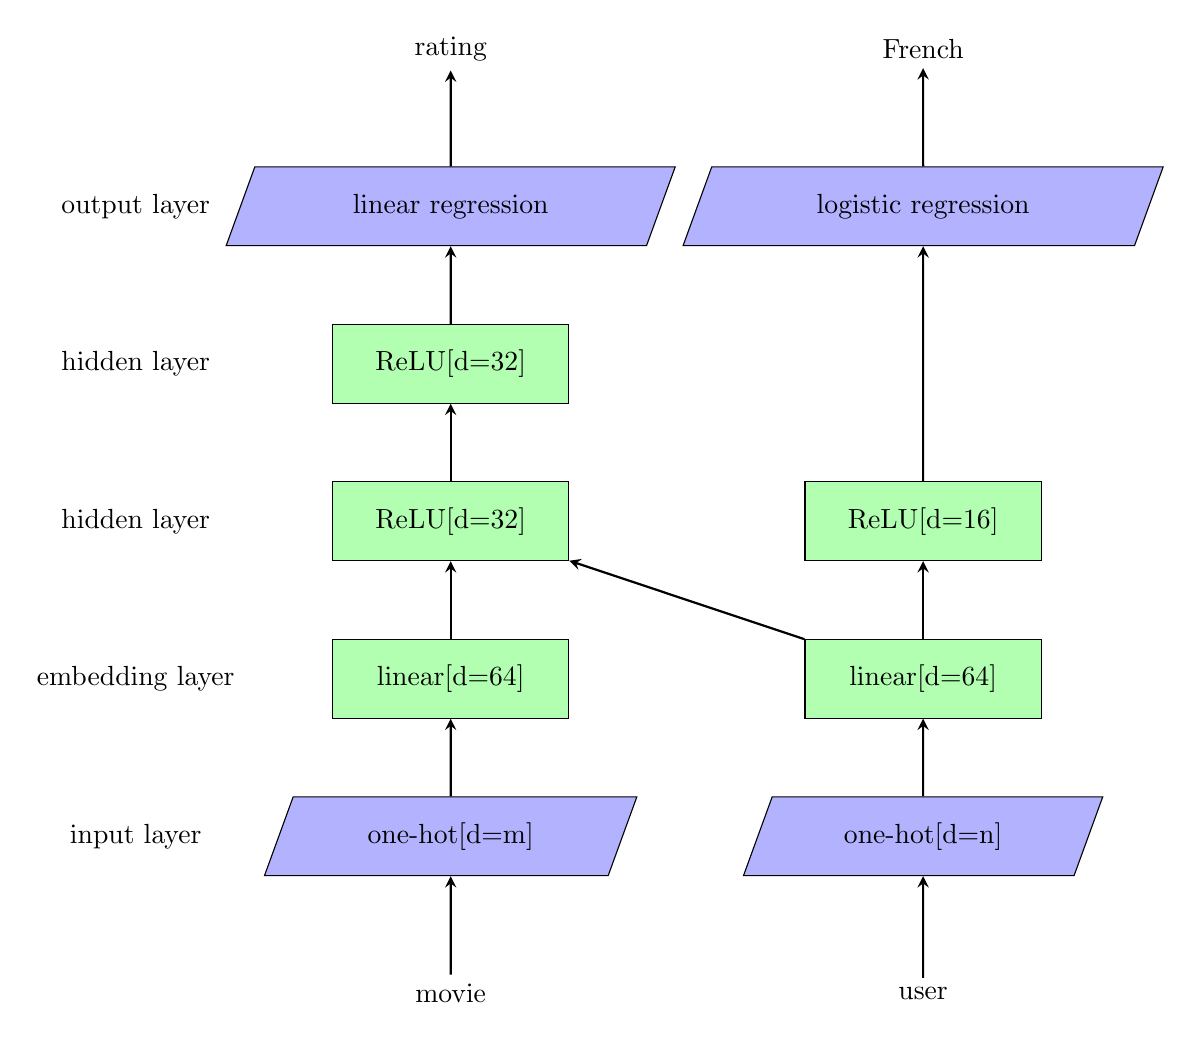
\begin{tikzpicture}[node distance=2cm]
	\tikzstyle{io} = [trapezium, trapezium left angle=70, trapezium right angle=110, minimum width=0cm, minimum height=1cm, text centered, draw=black, fill=blue!30]
	\tikzstyle{process} = [rectangle, minimum width=3cm, minimum height=1cm, text centered, draw=black, fill=green!30]
	\tikzstyle{arrow} = [thick,->,>=stealth]
	\node (linearRegression) [io] {linear regression};
	\node (logisticRegression) [io, right of=linearRegression, xshift=4cm] {logistic regression};
	\node (relu1) [process, below of=logisticRegression, yshift=-2cm] {ReLU[d=16]};
	\node (relu2) [process, below of=linearRegression] {ReLU[d=32]};
	\node (relu3) [process, below of=relu2] {ReLU[d=32]};
	\node (linear1) [process, below of=relu1] {linear[d=64]};
	\node (linear2) [process, below of=relu3] {linear[d=64]};
	\node (oneHot2) [io, below of=linear1] {one-hot[d=n]};
	\node (oneHot1) [io, below of=linear2] {one-hot[d=m]};
	\node (rating) [above of=linearRegression] {rating};
	\node (french) [above of=logisticRegression] {French};
	\node (output) [left of=linearRegression, xshift=-2cm] {output layer};
	\node (hidden2) [below of=output] {hidden layer};
	\node (hidden1) [below of=hidden2] {hidden layer};
	\node (embedding) [below of=hidden1] {embedding layer};
	\node (input) [below of=embedding] {input layer};
	\node (movie) [below of=oneHot1] {movie};
	\node (user) [below of=oneHot2] {user};
	\draw [arrow] (movie) -- (oneHot1);
	\draw [arrow] (user) -- (oneHot2);
	\draw [arrow] (oneHot2) -- (linear1);
	\draw [arrow] (oneHot1) -- (linear2);
	\draw [arrow] (linear1) -- (relu1);
	\draw [arrow] (linear1) -- (relu3);
	\draw [arrow] (linear2) -- (relu3);
	\draw [arrow] (relu3) -- (relu2);
	\draw [arrow] (relu1) -- (logisticRegression);
	\draw [arrow] (relu2) -- (linearRegression);
	\draw [arrow] (linearRegression) -- (rating);
	\draw [arrow] (logisticRegression) -- (french);
	\end{tikzpicture}	
	\caption{The multi-task prediction model with movie set size m, user set size n, embedding size 64: the model consists of 5 layers - an input layer with one-hot activation, an embedding layer of linear units, 2 hidden layers of rectified linear unites and an output layer of a linear regression unit and a logistic regression unit. The units in each layer are not shown. The d in the bracket refers to dimension, the layer's size (number of units in the layer).}
	\label{fig:multiTask}
\end{figure}

\subsubsection{Loss function}
I use hinge loss for logistic regression:
\begin{equation}
loss = l(t, y) = max(0, 1 - ty)
\end{equation}
where t is the expected output provided by the training data, y is the actual output predicted by the model, boolean values true and false are converted to numerical values 1 and -1. And I use squared error for linear regression:
\begin{equation}
	loss = l(t, y) = (t - y)^2
\end{equation}

\subsubsection{Learning algorithm}
I use the standard learning algorithm for neural net: stochastic gradient descent with back propagation. However, there are 2 types of training samples:
\begin{enumerate}
	\item x = (movie, user), y = (rating): in this case, the output and hidden layers on French side are deactivated as there is no supervision for them;
	\item x = (user), y = (French): in this case, all layers on the rating side are deactivated as there is no supervision for them;
\end{enumerate}
The model has the same structure and forward propagation in the prediction stage.

\subsection{Application scenario: link prediction}
The link prediction task mentioned in the QE is similar to the application scenario discussed above, and can use the same model with a few modifications:
\begin{enumerate}
	\item the numerical link attribute rating is replaced by a boolean link attribute connectivity (true if 2 nodes are connected, false otherwise);
	\item the linear regression unit for rating prediction is replaced by logistic regression unit for connectivity prediction;
	\item the training data will need negative samples randomly generated from the graph(the training set needs to contain similar amount of positive training samples (connected user pairs) and negative training samples (disconnected user pairs);
\end{enumerate}

\section{Conclusions}
I summarize node embedding, a neural net approach for learning vector representations of nodes in a graph. This process converts relational data to numerical data so that neural net can use them directly to perform various prediction tasks. The learning algorithm is on-line so it works well with streaming graph. I also introduce a new node embedding approach to address the weaknesses in the summarized approach. Specifically, the new approach has strengths of low complexity, comprehensive learning and multi-task prediction.

\bibliographystyle{acm}
\bibliography{references}

\end{document}
